\chapter[Introduction]{Project Introduction}
\label{cp:introduction}

\parindent0pt

\section{Vision \& Motivation}
\label{sec:vision}

In the first hours after an earthquake, the chance of pulling a trapped person out alive falls quickly. Ground teams
cannot see into collapsed blocks, streets are filled with debris, and the communication infrastructure is often down.
Small multirotor drones are an obvious way to help: they are cheap, fast to deploy, and can look into places a person
cannot reach. A \emph{fleet} of drones can search a district much faster than one drone. But a fleet only helps if the
drones divide the work sensibly, share what they find, and do not fly into buildings or into each other.

Two features of a real disaster make this hard, and both are at the core of the \emph{Multi-Agent Systems} course:

\begin{itemize}
  \item \textbf{No centre.} There is no control tower and no map. Each drone decides for itself from its own camera
        and from messages relayed by neighbours over a short-range, lossy radio. Coordination must emerge from local
        rules: consensus, distributed task allocation and information spreading.
  \item \textbf{No guaranteed honesty.} Some drones may malfunction or be compromised, for example by a spoofed
        navigation sensor, corrupted firmware or a hijacked radio. Such a drone can report a wrong position, claim to
        have searched an area it never visited, and stay silent about the people it sees. In the language of the
        course it is a \emph{Byzantine} agent~\citep{Lamport1982}.
\end{itemize}

The textbook defence against Byzantine agents in networked control is \emph{resilient consensus}. The Weighted
Mean-Subsequence-Reduced (W-MSR) algorithm~\citep{LeBlanc2013} discards the $F$ most extreme values a drone hears
before averaging, so that up to $F$ liars cannot drag the honest drones outside the range of honest values. This
protects the \emph{numbers} a fleet averages. Our starting observation is that it does not protect the
\emph{decisions} a search fleet makes:

\begin{enumerate}
  \item A \textbf{careful liar is never trimmed}. If it keeps its reported values inside the honest range, W-MSR keeps
        them, so filtering neither removes nor detects it.
  \item \textbf{Claims are not numbers}. ``I searched this block and nobody is there'' has nothing to average. A
        filtering fleet that believes this claim never revisits the block, and every survivor inside it is lost.
\end{enumerate}

\begin{keybox}[Thesis]
\emph{The filtering that makes a fleet resilient also makes it ignorant.} A drone should take risky actions, such as
declaring an area searched or flying into a gap, only on what it \textbf{knows}, meaning what holds in every possible
world about who the liar is, and not on what it is merely \textbf{told}. We build such a fleet and measure the
trade-off.
\end{keybox}

\begin{figure}[t]
    \centering
    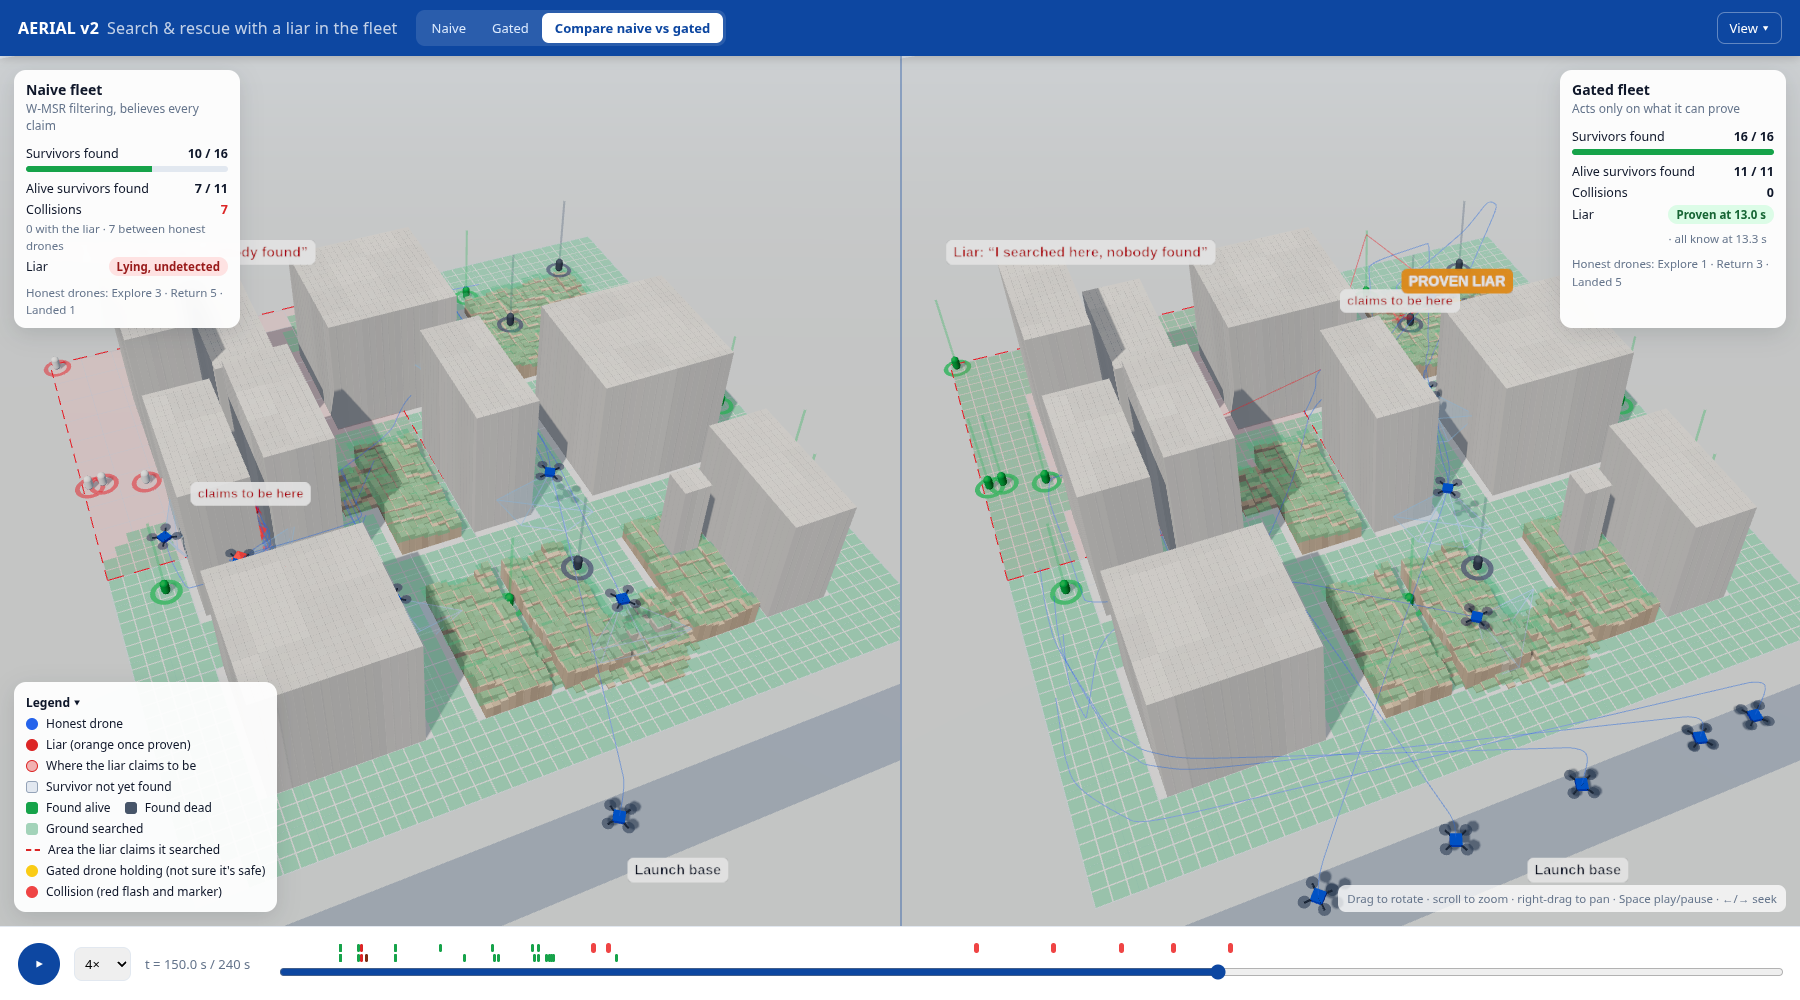
\includegraphics[width=\linewidth]{Figures/results/replay_compare.png}
    \caption[The VeriFly 3D replay: naive vs.\ gated fleet on the same mission]{The VeriFly 3D replay of one
    mission, 150\,s after take-off. Both fleets fly the same district with the same liar (red/orange drone), which
    claims the dashed corner as ``searched, nobody here''. \textbf{Left:} the W-MSR (\emph{naive}) fleet believes the
    claim; the survivors in the corner (red rings) are never found. \textbf{Right:} the \emph{gated} fleet proves
    the liar lied 0.8\,s after it starts lying, reopens the corner and finds all 16 survivors (green: found alive,
    grey: found dead).}
    \label{fig:teaser}
\end{figure}

\section{Goals}
\label{sec:goals}

The project has one scientific goal and several engineering goals that serve it.

\textbf{Scientific goal.} \emph{Quantify the price and the value of acting on knowledge instead of belief} in a
decentralised search-and-rescue fleet with up to $F$ lying members. Measure, under identical conditions, how many
survivors each trust policy finds, how safely it flies, how quickly it identifies the liar, and how long the mission
takes.

\textbf{Objectives.} These were fixed in the proposal and refined during the build:

\begin{table}[h]
\centering
\renewcommand{\arraystretch}{1.25}
\begin{tabularx}{\linewidth}{@{}l X X@{}}
\toprule
\textbf{ID} & \textbf{Objective} & \textbf{How it is met (where in this report)} \\
\midrule
O1 & A faithful, decentralised simulation: unmapped 3D terrain, a limited camera, a lossy multi-hop radio, and no
     agent ever reading the ground truth & Simulator architecture and enforced information boundary
     (\autoref{sec:system-model}, \autoref{sec:architecture}) \\
O2 & A complete mission: transit in formation, exploration with dynamic work division, survivor confirmation, return
     and landing & Mission state machine, geodesic Voronoi partition (\autoref{sec:mission}) \\
O3 & Resilient numeric coordination & W-MSR in formation and survivor localisation
     (\autoref{sec:wmsr}, \autoref{sec:res-localisation}) \\
O4 & Identify liars with \emph{zero} false accusations & S5 possible worlds and sound proof rules R1--R6
     (\autoref{sec:epistemic}, Proposition~\ref{prop:soundness}) \\
O5 & Never act unsafely on unverified claims & Provenance-tagged maps and the knowledge gate
     $\Kn_i\mathit{Safe}$ (\autoref{sec:gate}) \\
O6 & A controlled, statistically sound comparison & Paired randomness, 1,460 server runs, 95\% intervals,
     Wilcoxon tests (\autoref{cp:Results}) \\
O7 & Ground the network assumptions in theory & $\lambda_2$ convergence and $(r,s)$-robustness studies
     (\autoref{sec:res-theory}) \\
\bottomrule
\end{tabularx}
\caption{Project objectives and where each is addressed.}
\label{tab:objectives}
\end{table}

\section{Contributions}
\label{sec:contributions-summary}

\begin{enumerate}
  \item \textbf{A knowledge-gated fleet.} Every drone separates \emph{belief} (someone not yet proven a liar said it),
        which it uses to share out work, from \emph{knowledge} (true in every world consistent with the evidence),
        which it requires before risky actions. Knowledge is computed exactly over all sets of at most $F$ liars.
  \item \textbf{Sound proofs of lying from physics.} Five rules (UWB range, speed, radio horizon, camera, audit) that
        an honest drone provably cannot trigger, plus two weaker kinds of evidence (shared ranges and accusations)
        that only prove ``one of these two lies'', which makes framing impossible by construction.
  \item \textbf{Provenance-tagged maps.} Every coverage, terrain and survivor claim carries a bitmask of the drones
        that vouched for it. When a liar is caught, every claim resting only on its word reverts automatically, and
        the dynamic partition re-sweeps the area with no special re-sweep code.
  \item \textbf{A fair, reproducible experimental framework.} The four fleets share all code and, per seed, all
        random draws. We report 1,460 runs on the departmental GPU server, a 3D web replay, and a set of theory
        studies from a first, 2D build.
\end{enumerate}

\section{Code and Media}
\label{sec:code}

All code, experiment scripts, raw results and figures are in the group repository: \repolink. The
repository README and \tcode{CONTEXT.md} explain how to run every experiment in this report. The interactive 3D replays
(\tcode{docs/media/viewer.html}, \tcode{viewer\_collisions.html}) are single HTML files that open in any browser.

\section{Organisation of the Report}

\autoref{cp:literature} reviews the literature on resilient consensus, epistemic logic, multi-robot coverage and
runtime verification. \autoref{cp:prelim} fixes notation and recalls the theory we build on. \autoref{cp:problem}
formulates the problem, describes the system and the epistemic layer, and proves its key properties.
\autoref{cp:Results} presents the simulation setup, the experiments and their results, and the limitations.
\autoref{cp:Conclusion} concludes. The appendices give the full parameter set and the reproduction recipe, and the
last page lists each member's individual contribution.
